Durante l\textquoteright{}attivit\`{a} di stage sono stati riassunti i requisiti specificati per il progetto in diagrammi dei casi d\textquoteright{}uso al fine di specificare nella maniera pi\`{u} chiara e semplice possibile le specifiche per il progetto. In questa sezione viene presentato il minimo indispensabile per far comprendere quello in cui consisteva il dominio del progetto.  

\subsection{Casi d\textquoteright{}uso}

\subsubsection[UC1: Scenario principale]{UC1: Scenario principale}
\begin{figure}[H]
\begin{center}
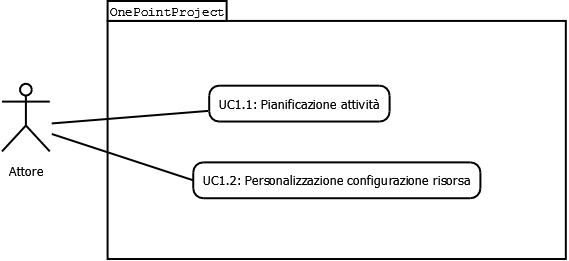
\includegraphics[width=0.80\textwidth]{img/UC/UC1.png}
\caption{UC1: Scenario principale}
\label{fig:UC1}
\end{center}
\end{figure}

\begin{description}
\item[Attori:]{utente autenticato al sistema.}
\item[Precondizione:]{Le infrastrutture di rete sono funzionanti e l\textquoteright{}applicativo \`{e} stato corretamente avviato.}
\item[Scenario principale:]{l\textquoteright{}utente pu\`{o} eseguire le seguenti operazioni:
	\begin{itemize}
	\item \textbf{pianificare le attivit\`{a}}: l\textquoteright{}utente dopo aver creato il progetto interessato o aperto in modifica uno esistente pu\`{o} utilizzare come strumento di pianificazione il WBS (UC1.1);
	\item \textbf{personalizzare la configurazione di una risorsa}: l\textquoteright{}utente accedendo al pannello di amministrazione risorse pu\`{o} scegliere come configurare una risorsa in termine di costi, sia interni che esterni, e di fascie orarie di lavoro e non (UC1.2).
	\end{itemize}}
\item[Postcondizione per successo:]{il sistema \`{e} in attesa di una scelta da parte dell\textquoteright{}utente.}
\end{description}

\subsubsection[UC1.1: Pianificazione attivit\`{a}]{UC1.1: Pianificazione attivit\`{a}}
\begin{figure}[H]
\begin{center}
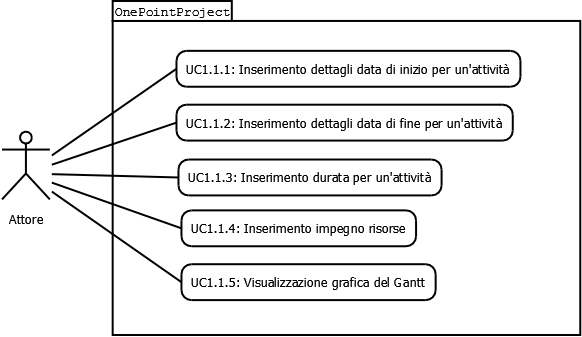
\includegraphics[width=0.80\textwidth]{img/UC/UC1.1.png}
\caption{UC1.1: Pianificazione attivit\`{a}}
\label{fig:UC1.1}
\end{center}
\end{figure}

\begin{description}
\item[Attori:]{utente autenticato al sistema.}
\item[Precondizione:]{L\textquoteright{}utente \`{e} in opzione modifica per un certo progetto e le infrastrutture di rete sono funzionanti.}
\item[Scenario principale:]{l\textquoteright{}utente pu\`{o} eseguire le seguenti operazioni:
	\begin{itemize}
	\item \textbf{inserire i dettagli relativi alla data di inizio dell\textquoteright{}attivit\`{a}}: l\textquoteright{}utente pu\`{o} inserire data e ora di inizio per un\textquoteright{}attivit\`{a} (UC1.1.1);
	\item \textbf{inserire i dettagli relativi alla data di fine dell\textquoteright{}attivit\`{a}}: l\textquoteright{}utente pu\`{o} inserire data e ora di fine per un\textquoteright{}attivit\`{a} (UC1.1.2);
	\item \textbf{inserire una durata per l\textquoteright{}attivit\`{a}}: l\textquoteright{}utente pu\`{o} inserire la durata dell\textquoteright{}attivit\`{a} nel formato dd-hh-mm che aggiorner\`{a} di conseguenza la data di fine, si tratta di un\textquoteright{}opzione alternativa all\textquoteright{}inserimento della data di fine (UC1.1.3);
	\item \textbf{inserire l\textquoteright{}impegno per le risorse coinvolte}: l\textquoteright{}utente dopo aver assegnato le risorse all\textquoteright{}attivit\`{a} interessata pu\`{o} scegliere le ore di lavoro della risorsa per l\textquoteright{}attivit\`{a} stessa (UC1.1.4);
	\item \textbf{visualizzazione del diagramma di Gantt}: l\textquoteright{}utente pu\`{o} visualizzare il diagramma di Gantt delle attivit\`{a} elencate nel WBS (UC1.1.5).
	\end{itemize}}
\item[Postcondizione per successo:]{il sistema aggiorna il WBS delle attivit\`{a} e in caso di salvataggio rende persitente la pianificazione effettuata.}
\end{description}

\subsubsection[UC1.2: Personalizzazione configurazione risorsa]{UC1.2: Personalizzazione configurazione risorsa}
\begin{figure}[H]
\begin{center}
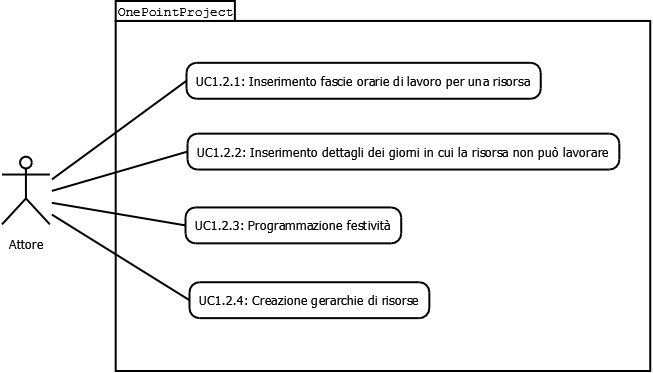
\includegraphics[width=0.80\textwidth]{img/UC/UC1.2.png}
\caption{UC1.2: Personalizzazione configurazione risorsa}
\label{fig:UC1.2}
\end{center}
\end{figure}

\begin{description}
\item[Attori:]{utente autenticato al sistema.}
\item[Precondizione:]{L\textquoteright{}utente ha i permessi per effettuare le modifiche alle risorse, ha quindi facolt\`{a} di accesso al pannello di amministrazione risorse e le infrastrutture di reste sono funzionanti.}
\item[Scenario principale:]{l\textquoteright{}utente pu\`{o} eseguire le seguenti operazioni:
	\begin{itemize}
	\item \textbf{inserire fascie orarie di lavoro per una risorsa}: l\textquoteright{}utente pu\`{o} inserire data e ora di inizio per un\textquoteright{}attivit\`{a} (UC1.2.1);
	\item \textbf{inserire i dettagli dei giorni in cui la risorsa \`{e} in stallo}: l\textquoteright{}utente pu\`{o} inserire data e facie orarie in cui la risorsa non pu\`{o} lavorare, pu\`{o} inoltre specificare le ragioni per cui la risorsa non pu\`{o} lavorare per esempio: manutenzione, locata a terzi ecc. (UC1.2.2);
	\item \textbf{programmare le festivit\`{a}}: l\textquoteright{}utente pu\`{o} indicare se una risorsa lavora o meno nei giorni festivi in base al calendario italiano (UC1.2.3);
	\item \textbf{creazione gerarchie di risorse}: l\textquoteright{}utente pu\`{o} specificare delle gerarchie di risorse tale che per una risorsa figlio \`{e} impostabile la possibilit\`{a} di ereditare o meno la configurazione del padre (UC1.2.4);
	\end{itemize}}
\item[Postcondizione per successo:]{il sistema aggiorna nel database le propriet\`{a} di configurazione delle risorse.}
\end{description}
